\section{Model and Preliminaries}
\label{sec: model}


We consider a central decision maker (platform) facing an online matching problem that evolves over a finite horizon of $T\geq1$ discrete time periods. The platform knows the set of supply vertices $\supply$ in advance. Demand vertices arrive one at a time in an on-line fashion, i.e., in each period $t = 1, \ldots, T$, a vertex $v_t$ arrives and the decision maker observes its type. The type of a demand vertex $v$ is defined through the vector ${(\prob_{u,v})}_{u\in \supply} \in [0,1]^{|\supply|}$,  where $\prob_{u,v}$ indicates the probability that a demand-side vertex $v \in V$ chooses to consume supply vertex $u \in \supply$ upon the decision maker matching $v$ to $u$. To simplify notation, and when clear from context, we usually refer to demand nodes by their arrival time $t$ and use $v_t$ to refer to the type of the $t$-th arrival. Throughout, we denote vectors in bold.


{At the beginning of period $t$, the platform observes the type of vertex $t$ and must choose whether to match vertex $t$ irrevocably to a supply-side vertex $u$ or leave $t$ permanently unmatched.
If the platform matches $t$ to $u$, $t$ chooses to consume $u$, \emph{and}  $u$ is still available (i.e., it has not been consumed before), then we refer to the match of $t$ and $u$ as a \textit{successful match} or a \textit{consumption} and refer to $u$ as a \emph{consumed supply node}. Otherwise, the match is not successful (either because $t$ chooses not to consume or because $u$ has already been consumed before) and no consumption occurs. That is, our model of stochastic rewards distinguishes between the platform matching demand node $t$ to $u$ and that match being successful (i.e., $t$ consuming $u$). }


\textbf{\emph{Algorithms.}}
The decision-maker's objective is to maximize the expected amount of supply that demand nodes consume over $T$ periods. As discussed before, our results aim to characterize the performance of \emph{delayed algorithms},
i.e., ones that only observe whether a match succeeded at the end of the time horizon. 
Formally, an algorithm $\alg$ describes a non-anticipating (possibly randomized) sequence of match decisions $\{
\mathbf{Y}_t
\}^T_{t
=1} $ for every $v_t\in V$, where $\mathbf{Y}_t
=(Y_{u,t})_{u \in \supply}$  and $Y_{u,t}$ is a random indicator variable that is~$1$ if and only if the arrival $v_t$ is matched to $u$ (regardless of whether the match is successful). Moreover, we define the random indicator variable $X_{u,t}$ that is $1$ if and only if the algorithm $\alg$  matches $t$ to $u$ \emph{and} the match is successful; we similarly define $\mathbf{X}_t
=(X_{u,t})_{u \in \supply}$. In other words, the indicator $Y_{u,t}=1$ stands for arrival $t$  having been matched to $u$ whereas $X_{u,t} = 1$ means that the match was successful, i.e., (i) $t$ was matched to $u$, (ii) $t$ chose to consume $u$, and (iii) $u$ has not been previously consumed.\footnote{As any feasible assignment algorithm matches each $t$ to at most one supply vertex $u\in \supply$ we have that, when $Y_{u,t}=1$, then  all remaining variables $X_{u',t}$ and $Y_{u',t}$ for $u' \in \supply\setminus\{u\}$ must be zero.} In our delayed setting, an algorithm is restricted to make decisions that \textit{cannot be based on the realization} of the random variables $(\mathbf{X}_{t'})_{t'=1}^{t-1}$. Rather, decisions can only be based on the previous matching decisions up to time $t$, $(\mathbf{Y}_{t'})_{t'=1}^{t-1}$. Formally, the stochastic process is $(\mathbf{Y}_{t})_{t=1}^{T}$ is $\mathcal{H}_t$-adapted,
where $\{\mathcal{H}_t\}_{t=1}^T$ is the filtration describing the algorithm's history. That is, letting $s$ be the algorithm's random
seed, we have $\mathcal{H}_1=\sigma(s, v_1)$ and  $\mathcal{H}_t=\sigma(\mathcal{H}_{t-1}, \mathbf{Y}_{t-1},  v_t)$ for every $t \in \{2, \ldots, t\}$,  where we use $v_t$ to denote the type of the $t$-th arrival. Throughout, we abuse notation by using $\alg$ to refer to both an algorithm and its value, when the intended meaning is clear from the context.

%\vspace{-.15in}
\subsubsection*{Arrival models,  competitive ratio, and imbalance.}
We derive results for two commonly studied demand arrival models: stochastic and adversarial. In the \textit{stochastic arrival model}, which we sometimes refer to as the stochastic setting, we are given a finite set $V$ of possible demand types and a probability distribution $\{p_{v}\}_{v \in V}$ over these types, from which each $v_t$ is drawn independently.  In the \textit{adversarial arrival model}, we are given a finite set $V$ of possible demand types and the probabilities of consumption are set to be equal, i.e. $\prob_{u,t} \in \{ 0, \prob\}$ for $\prob \in (0,1]$ where $\prob$ can be instance-dependent but we do not make any additional assumptions over the arrivals, other than their types being in a generic set $V$ and that for any demand node $v\in V$ there exists $u\in $ such that $\prob_{u,v}=\prob$. For either arrival model, we call the set of $u$ such that $\prob_{u,v}>0$ the neighborhood of $v$ and denote it by  $N(v) = \{u \in \supply : \prob_{u,v} > 0 \}$. For the adversarial model, we also define the set $E=\{(u,t): u\in \supply, t\in V, \mu_{u,t}=\mu\}$.

Our results rely on the notion of CRs to evaluate the performance of delayed algorithms. To that end, we start by defining an instance. An instance $\inst$ is composed of the set $\supply$ of supply vertices $\supply$, a set of potential demand nodes $V$, and the consumption probabilities $\{ \prob_{u,v}\}_{u \in \supply, v \in V} \subseteq (0,1)^{\supply \times V}$ associated with each type $v \in V$.  In the stochastic arrivals settings, we assume that the instance also contains the probability distribution $\{p_v\}_{v \in V}$ over the demand-side arrival types. We slightly abuse notation and use $\inst$ to denote an instance for either arrival model.  
In the stochastic arrivals setting, the \textit{expected value} of an algorithm $\alg$ given instance $\inst$, $\mathbb{E}[\alg(\inst)]$ refers to the expected value of $\alg$ under stochastic arrivals where the expectation is taken over the sequence of arrivals, the (possibly random) decisions of the algorithm, and the consumption realizations. On the other hand,  in the adversarial setting, we instead define the expected value of an algorithm given an instance and an arrival sequence. That is, the expected value of an algorithm $\alg$ given instance $\inst$ and an arrival sequence  {$\sigmabf=(1, \ldots, T)$} is denoted by $\mathbb{E}[\alg(\inst, \sigmabf)]$, where the expectation is taken over the possibly random decisions of the algorithm and the consumption realizations. 
%\vspace{-.7em}

\begin{figure}[h]
\centering
\tikzset{every picture/.style={line width=0.75pt}} %set default line width to 0.75pt        

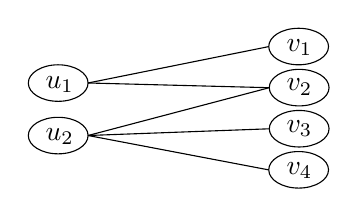
\begin{tikzpicture}[x=0.75pt,y=0.75pt,yscale=-.55,xscale=.9]
%uncomment if require: \path (0,310); %set diagram left start at 0, and has height of 310

%Shape: Circle [id:dp705325080636104] 
\draw   (237.14,68.73) .. controls (237.17,77.56) and (230.04,84.76) .. (221.2,84.79) .. controls (212.37,84.83) and (205.17,77.7) .. (205.14,68.86) .. controls (205.1,60.02) and (212.23,52.83) .. (221.07,52.79) .. controls (229.91,52.76) and (237.1,59.89) .. (237.14,68.73) -- cycle ;
%Shape: Circle [id:dp9045264439682683] 
\draw   (236.86,32.73) .. controls (236.9,41.56) and (229.76,48.76) .. (220.93,48.79) .. controls (212.09,48.83) and (204.9,41.7) .. (204.86,32.86) .. controls (204.82,24.03) and (211.96,16.83) .. (220.79,16.8) .. controls (229.63,16.76) and (236.82,23.89) .. (236.86,32.73) -- cycle ;
%Shape: Circle [id:dp7330157492007956] 
\draw   (108.14,64.73) .. controls (108.17,73.56) and (101.04,80.76) .. (92.2,80.79) .. controls (83.37,80.83) and (76.17,73.7) .. (76.14,64.86) .. controls (76.1,56.02) and (83.23,48.83) .. (92.07,48.79) .. controls (100.91,48.76) and (108.1,55.89) .. (108.14,64.73) -- cycle ;
%Shape: Circle [id:dp6777718508352495] 
\draw   (236.86,140.73) .. controls (236.9,149.56) and (229.76,156.76) .. (220.93,156.79) .. controls (212.09,156.83) and (204.9,149.7) .. (204.86,140.86) .. controls (204.82,132.03) and (211.96,124.83) .. (220.79,124.8) .. controls (229.63,124.76) and (236.82,131.89) .. (236.86,140.73) -- cycle ;
%Shape: Circle [id:dp5798086220020264] 
\draw   (237.14,104.73) .. controls (237.17,113.56) and (230.04,120.76) .. (221.2,120.79) .. controls (212.37,120.83) and (205.17,113.7) .. (205.14,104.86) .. controls (205.1,96.02) and (212.23,88.83) .. (221.07,88.79) .. controls (229.91,88.76) and (237.1,95.89) .. (237.14,104.73) -- cycle ;
%Shape: Circle [id:dp6665288116424322] 
\draw   (108.14,110.73) .. controls (108.17,119.56) and (101.04,126.76) .. (92.2,126.79) .. controls (83.37,126.83) and (76.17,119.7) .. (76.14,110.86) .. controls (76.1,102.02) and (83.23,94.83) .. (92.07,94.79) .. controls (100.91,94.76) and (108.1,101.89) .. (108.14,110.73) -- cycle ;
%Straight Lines [id:da6695348841913797] 
\draw    (108.14,64.73) -- (204.86,32.86) ;
%Straight Lines [id:da13011748270531487] 
\draw    (108.14,64.73) -- (205.14,68.86) ;
%Straight Lines [id:da41568081525275913] 
\draw    (108.14,110.73) -- (205.14,68.86) ;
%Straight Lines [id:da387934327631003] 
\draw    (108.14,110.73) -- (205.14,104.86) ;
%Straight Lines [id:da9311827336887017] 
\draw    (108.14,110.73) -- (204.86,140.86) ;

% Text Node
\draw (213,59) node [anchor=north west][inner sep=0.75pt]   [align=left] {{$v_2$}};
% Text Node
\draw (213,24) node [anchor=north west][inner sep=0.75pt]   [align=left] {{$v_1$}};
% Text Node
\draw (213,132) node [anchor=north west][inner sep=0.75pt]   [align=left] {{$v_4$}};
% Text Node
\draw (213,95) node [anchor=north west][inner sep=0.75pt]   [align=left] {{$v_3$}};

% Text Node
\draw (84,57) node [anchor=north west][inner sep=0.75pt]   [align=left] {{$u_1$}};
% Text Node
\draw (84,102) node [anchor=north west][inner sep=0.75pt]   [align=left] {{$u_2$}};

\end{tikzpicture}
\caption{Depending on $\prob\in\{1/4,.5,1\}$ the instance is $1/2$-oversupplied, balanced, or $2$-undersupplied.}\label{fig:example_imbalance}
\end{figure}

We measure an algorithm's performance through its CR relative to the following LP benchmark (with $\market=1$),\footnote{As it is common in the literature on online matching with stochastic rewards, we  compare the performance of $\alg$ with the LPs to maintain tractability; towards the end of this section we discuss alternative benchmark choices.}
and let $x_{u, v}$ capture the fraction of demand node $v$ that is assigned to supply node~$u$.
\begin{minipage}[t]{0.47\textwidth}
\centering $\offIkappa$ \textbf{(Adversarial)}
\begin{align}
    \max_{\mathbf{x}\geq \mathbf{0}} \quad & \sum_{(u, t) \in E}{ \prob \cdot x_{u, t}} \notag\\
    \textrm{s.t.} \quad & \sum_{t: (u,t) \in E } \prob \cdot  x_{u, t} \leq \market, \quad && \forall u \in \supply \label{adversarial_lp: kappa-constraint}\\
    & \sum_{u: (u,t) \in E} x_{u, t} \leq 1, \quad && \forall t \in [T] \label{adversarial_lp: demand_constraint}
\end{align}
\end{minipage}%
\hspace{.4em}
\begin{minipage}[t]{0.47\textwidth}
\centering $\offIkappa$ \textbf{(Stochastic)}
\begin{align}
     \max_{\mathbf{x}\geq \mathbf{0}} \quad & \sum_{u\in \supply, v\in V}{ \prob_{u,v} \cdot x_{u, v}} \notag\\
    \textrm{s.t.} \quad & \sum_{v \in V} \prob_{u,v} \cdot  x_{u, v} \leq \market, \quad && \forall u \in \supply \label{stochastic_lp: kappa-constraint}\\ 
    & \sum_{u \in \supply} x_{u, v} \leq T p_v, \quad && \forall v \in V \label{stochastic_lp: demand_constraint}
\end{align}
\end{minipage}

Superficially, the parametrization of these LPs by $\market$ resembles the $b$-matching formulations in the literature \citep{kalyanasundaram2000optimal}, though we use them to define imbalance below. Throughout, we denote by $\offI(\inst) = \offI(\inst, 1)$ the optimal value of the respective linear program for either arrival setting (note that the adversarial arrival model requires no dependence on~$\sigmabf$, because the linear program is unaffected by the arrival order of the demand nodes). Each summand in the objective function of $\offI(\inst)$, in either LP, rewards a solution fractionally for assigning $v$ to $u$ with a coefficient that captures the probability that $v$ would consume $u$. With $\market=1$, constraints (\ref{adversarial_lp: kappa-constraint}) and (\ref{stochastic_lp: kappa-constraint}) capture that each supply node $u$ can be consumed at most once. Lastly, constraint (\ref{adversarial_lp: demand_constraint}) stipulates that any demand node $v$ can be matched at most once under adversarial arrivals; similarly, in the stochastic setting, the upper bound in (\ref{stochastic_lp: demand_constraint})  is the expected number of times a node of type $v$ appears in the arrival sequence. In \Cref{proof: offline is upper bound} we prove the following lemma asserting that the LPs are valid upper bounds for any algorithm. 

\begin{lemma}
    \label{lemma: offline is upper bound}
    Let $\inst$ be an instance and $\alg$ be any algorithm with $(X_{u,t})_{u \in \supply, t \in [T]}$ the sequence of matching decisions that where successful. Then, in either setting,
    $\offI(\inst) \geq  \mathbb E\left[\sum_{ (u,t) \in \supply \times [T]} X_{u,t} \right]$.
\end{lemma}



We now define the following notion of CR as our performance metric.


\begin{definition}%[Competitive Ratio]
Let $\comp \in [0,1]$ and $\mathcal{F}$ be a family of instances for the stochastic arrivals setting; an algorithm $\alg$ is said to be \textit{$\comp$-competitive for family $\mathcal{F}$} if
% \begin{equation*}
$        \inf_{\inst \in \mathcal{F}}{\mathbb E[\alg(\inst)] }/{\offI(\inst)} \geq \comp$.
%    \end{equation*}
    Similarly, for a family of instances in the adversarial setting, $\mathcal{F}$,  an $\alg$ is $\comp$-competitive for $\mathcal{F}$ if
    % \begin{equation*}
        $\inf_{\inst \in \mathcal{F}} \inf_{\sigmabf} \frac{\mathbb E[\alg(\inst, \sigmabf)] }{\offI(\inst)} \geq \comp$.
    % \end{equation*}
\end{definition}

When the family of instances $\mathcal{F}$ is not specified, we refer to $\mathcal{F}$ as the set of all possible instances. However, we usually parameterize instances based on the demand-supply imbalance as we discuss next.

\textbf{\emph{Oversupplied and Undersupplied Instances.}}
Our findings include sharp characterizations of how supply-demand imbalances affect the performance of online algorithms. The example in Figure \ref{fig:example_imbalance} motivates our characterization of imbalanced instances. The figure displays an instance with 2 supply nodes and 4 demand nodes; with  $\prob_{uv}=\frac{1}{2} \, \forall u\in \supply,v\in V$, it is natural to think of this instance as a \emph{balanced} one. Indeed, there exists an assignment ($v_1,v_2$ to $u_1$ and $v_3,v_4$ to $u_2$) under which the expected demand realizing at each supply node is exactly 1 and there exists no assignment under which the expected demand realizing at each supply node is greater 1. In contrast, with $\prob_{uv}=1 \, \forall u\in \supply,v\in V$, we would view the instance with the same nodes as undersupplied; in particular, with the same assignment as before we would now be assigning 2 (expected) demand to every supply node. In that regard, it is natural to think of the instance with with $\prob_{uv}=1 \, \forall u\in \supply,v\in V$ as 2-undersupplied, which captures that if we had twice as much supply at each supply node the instance would be balanced. Finally, suppose we had  $\prob_{uv}=\frac{1}{4} \, \forall u\in \supply,v\in V$; then, the same assignment as before we would now be assigning just $1/2$ (expected) demand to every supply node. In that regard, it is natural to think of the instance with with $\prob_{uv}=1/4 \, \forall u\in \supply,v\in V$ as $1/2$-oversupplied, which captures that there exists an assignment under which the expected demand at each supply node is $1/2$ and there exists no assignment under which the expected demand at each supply node is larger.

We generalize these intuitions to arbitrary graphs through the parameter $\market$ in the definition of $\offIkappa$. The resulting LPs

connect with our example from Figure \ref{fig:example_imbalance} as follows: in our 2-undersupplied instance we find that $\offIkappa=\kappa \cdot \offI(\inst)$ for $\kappa=2$, i.e., as we increase $\kappa$ to loosen the supply constraint the objective increases, least up to $\kappa=2$, linearly in $\kappa$. In contrast, in our $1/2$-oversupplied instance, as we decrease $\kappa$ to tighten the supply constraint the objective remains the same down to $\kappa=1/2$. To capture this phenomenon we define $\kappa$ under- and oversupplied instances as follows: 
\begin{definition} \label{def: under/oversupplied}
We call an instance $\inst$: 
(1) \textit{$\market$-undersupplied} if $\market = \max\{ \overline{\market} \geq 1 \colon \offI(\inst, \overline{\market}) = \overline{\market} \cdot \offI(\inst)\}$, (2) \textit{$\market$-oversupplied} if $
            \market = \min\{ \overline{\market} \leq 1 \colon \offI(\inst,\overline{\market}) = \offI(\inst)\}$, and (3) 
         \textit{balanced} if it is both $1$-oversupplied and $1$-undersupplied.
    \end{definition}
Observe that $\market=1$ is an element of the sets in the definition, guaranteeing that the sets are non-empty. We make the technical assumption that the value of the maximum for $\market$-undersupplied instances and the minimum for $\market$-oversupplied instances, as defined in Definition \ref{def: under/oversupplied}, is attained at rational numbers. Intuitively, an instance is $\market$-undersupplied if the respective offline problem with capacity $\market$ has exactly $\market$ times the same value as the problem with capacity $1$. An instance is $\market$-oversupplied if the offline problem with capacity $\market$ is equal to the offline problem with capacity~1.

A direct consequence of \Cref{lemma: offline is upper bound} is that $\offIkappa/\market$ provides an upper bound to the expected value of any online algorithm on a $\market$-undersupplied instance. Analogously, if an instance is $\market$-oversupplied for $\kappa < 1$, then $\offIkappa$ provides an upper bound to the expected value of any online algorithm.

\subsection*{Discussion of modeling assumption}

\paragraph{Definition of imbalance.}

The advantage of our imbalance definition (\Cref{def: under/oversupplied}) is its intuitive  interpretability; on undersupplied instances one may achieve a higher objective by increasing the capacity of all the supply nodes and on oversupplied instances one maintains the objective when reducing the capacity of all the supply nodes. However, a practical limitation of our definition is that it may suggest that many instances are balanced even though they seem (intuitively) imbalanced. In particular, this holds true when a graph is locally under- and locally oversupplied: \Cref{def: under/oversupplied} treats such graphs as balanced as they are neither \emph{globally} undersupplied nor oversupplied. To address this limitation, we propose the following alternative definition of imbalance:

\begin{definition}
    \label{def: new_over_undersupplied}
    Let $\inst$ be a given instance. For $\market \geq 1$ we say that the tuple  $(\undersup, \oversup)$ is a $\market$-imbalanced pair if it fulfills the following conditions:
    \begin{enumerate}[(i)]
        \item (Partition) $\undersup$ and $\oversup$ are disjoint and $\undersup \cup \oversup = \supply$.
        \item (Undersupplied set) If the capacity of every node in $\undersup$ gets augmented by $\market$, then the offline solution grows by $(\market-1) | \undersup|$. In other words,
        \begin{align*}
             &\offI(\inst) + (\market-1)|\undersup| = \max_{\mathbf{x}\geq \mathbf{0}} \quad  \sum_{(u, t) \in E}{ \prob \cdot x_{u, t}} \tag{$\offI^{\undersup, \mathcal O}(\inst, \market)$} \label{prob: offlineUndersupplied}\\
    \mathrm{s.t.} \quad & \sum_{t: (u,t) \in E } \prob \cdot  x_{u, t} \leq \market \quad  \forall u \in \undersup, 
    \quad \sum_{t: (u,t) \in E } \prob \cdot  x_{u, t} \leq 1 \quad \forall u \in \oversup,
    \quad \sum_{u: (u,t) \in E} x_{u, t} \leq 1 \quad  \forall t \in [T].
        \end{align*}
        
        \item (Oversupplied set) There exists an optimal solution $\mathbf{x}^*$ to $\offI(\inst)$ that uses at most $1/\market$ capacity at nodes in $\oversup$. In other words, there exists $\mathbf{x}^*$ optimal solution to $\offI(\inst)$ that satisfies $\prob \sum_{t: (u,t)} x_{u,t}^* \leq 1/\market$ for all $u \in \mathcal O$.
    \end{enumerate}
\end{definition}

Under this new definition, we can provide an analogous CR result for adversarial arrivals as long as the algorithm knows which nodes are in $\oversup$ and which nodes are in $\undersup$.

In practice, even under adversarial arrivals, platforms can likely use historical data to determine which nodes belong to the under- or oversupplied sets (\Cref{sec: alternative_def} contains a method to compute these for offline instances). For instance, in spatial settings (ridehailing, volunteer matching), some neighborhoods are consistently over- or undersupplied during certain hours. Similarly, in refugee resettlement some locations offer consistently higher employment probabilities and matching optimization would thus consistently use all of their capacity, but not that at locations with lower probabilities. Though we do not capture the intricacies of these applications, these examples illustrate practical settings in which platforms would reasonably know $\oversup$ and $\undersup$.


\paragraph{Choice of Benchmark.} 
{Most of the recent literature on online matching with stochastic rewards has used tighter benchmarks than the standard matching LP, $\offI$. With these benchmarks, including the Configuration LP by \citet{huang2020online}, the Path Based Program by \citet{goyal2023online} for adversarial arrivals, and the benchmark of \citet{brubach2020online}  for stochastic arrivals, authors have been able to achieve better CRs than possible vis-a-vis $\offI$. However, for our purposes, these benchmarks come with a significant disadvantage: as they add exponentially many constraints to the linear program, it is challenging to compute their objective value even for instances with relatively few nodes and edges (see Appendix \ref{ssec: pbp_infeasible}). This added complexity makes it impractical to compute the tighter upper bound on an instance's objective values, whereas $\offI$ offers a computationally feasible approach. Moreover, due to its compactness, $\offI$ yields a more interpretable benchmark that lends easily lends itself to the study of imbalanced instances. Motivated by these advantages, we choose to follow the more traditional benchmark $\offI$ to evaluate the performance of our algorithms, thereby sacrificing potentially tighter CRs for gains in tractability and interpretability. Nonetheless, some of our numerical results (see Appendix \ref{ssec:imbalanced}) also explore the performance of some of these newer algorithms under imbalanced instances.

